\documentclass[12pt,a4paper]{journal}
\usepackage[margin=1in]{geometry}

\usepackage{times}

\usepackage[utf8]{inputenc}
\usepackage[T1]{fontenc}
\usepackage{indentfirst}
\usepackage{amsmath}
\usepackage{amsfonts}
\usepackage{amssymb}
\usepackage{caption}
\usepackage{subcaption}
\usepackage{graphicx}
\usepackage{siunitx}
\sisetup{range-phrase=--, range-units=single}

\graphicspath{{img/}}
\usepackage[numbers, super, sort&compress]{natbib}

\begin{document}

\section*{Retinal haemodynamics, vascular diseases, neovascular age-related macular degeneration and diabetic retinopathy}

\subsection*{Retinal haemodynamics}

\begin{figure}[t]
  \centering
  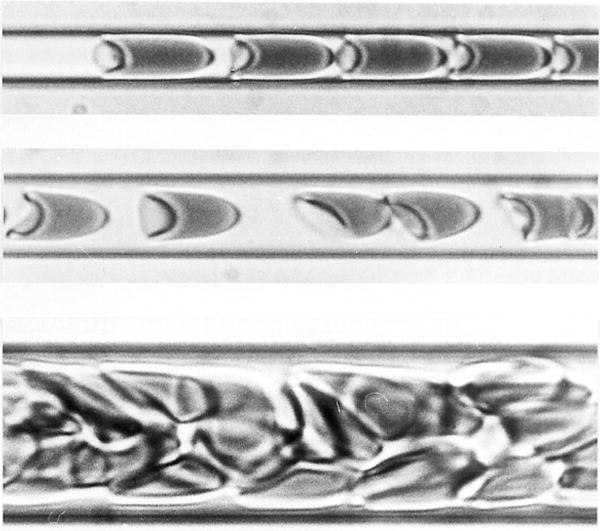
\includegraphics[width=0.45\textwidth, height=5.3cm]{cropped-RBC-in-capillaries.jpg}
  \hfill
  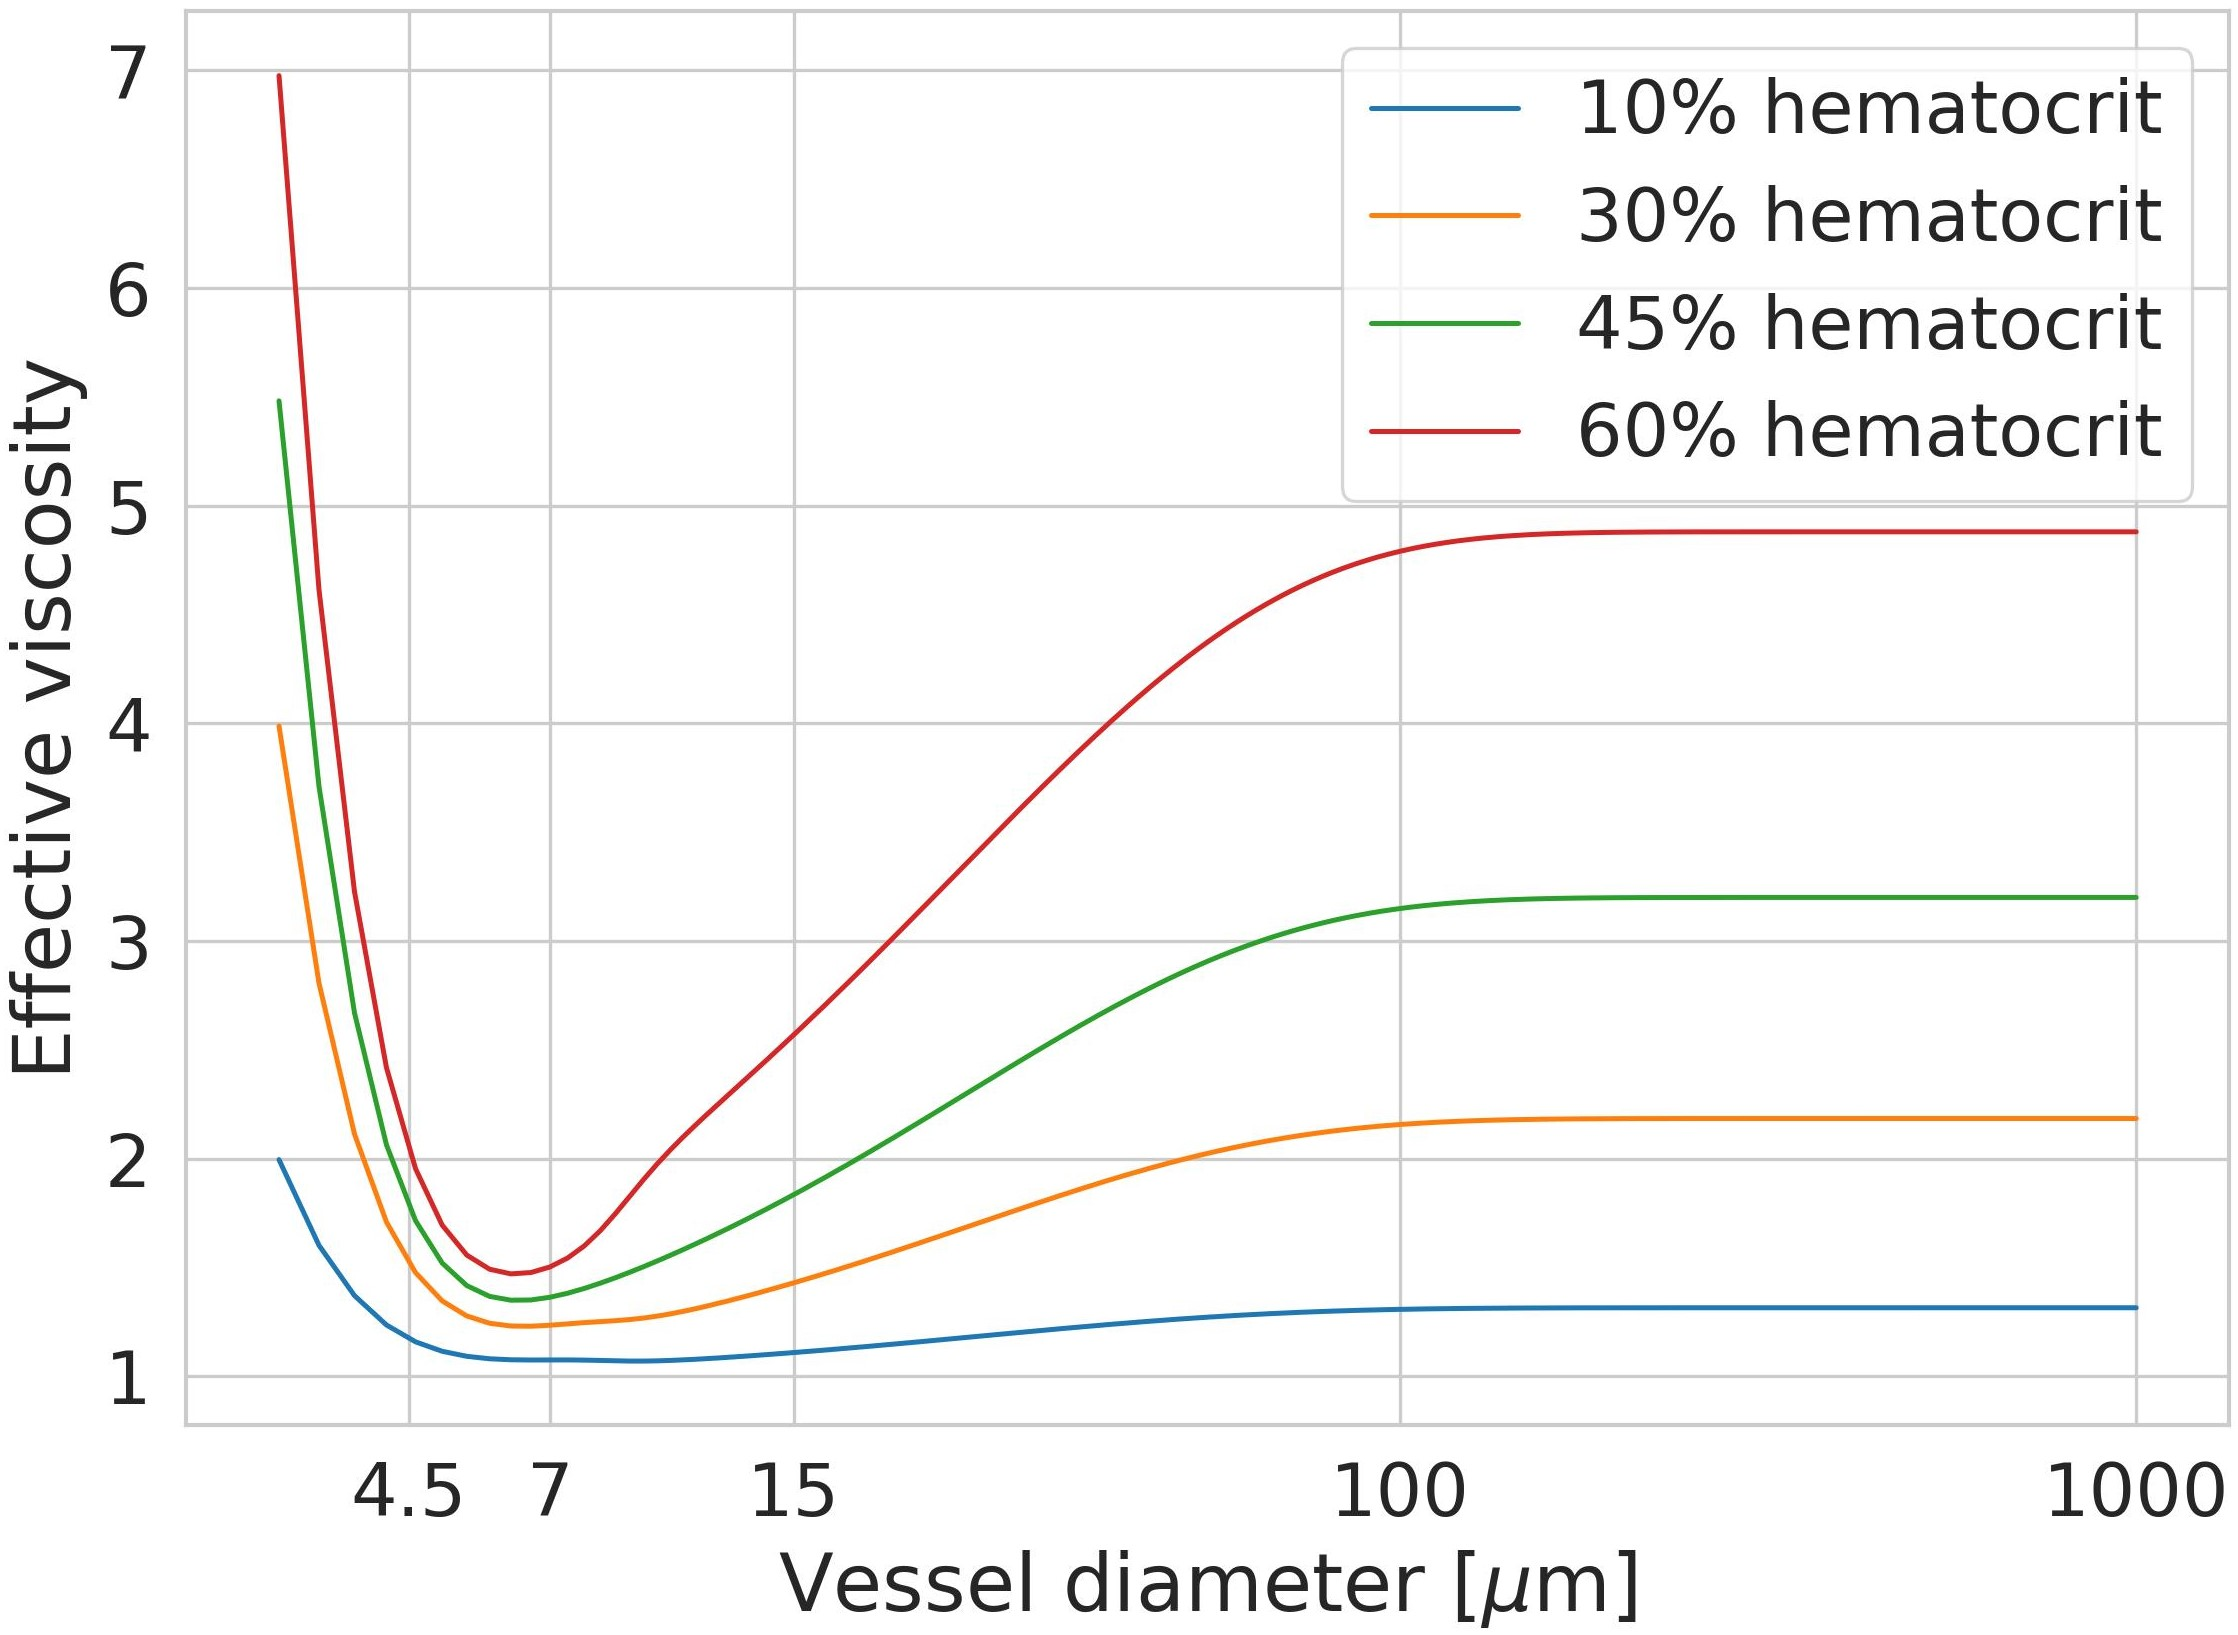
\includegraphics[width=0.45\textwidth, height=5.3cm]{EffectiveViscosity-Secomb.jpeg}
  \caption{Example of the effect of capillary calibre on the flow of blood. \textbf{Left}: Red blood cells in suspension in blood flowing within tubes of different diameter: \SI{4.5}{\micro\meter} (top), \SI{7}{\micro\meter} (middle) and \SI{15}{\micro\meter} (bottom). One can observe the flow of cells converging into a single file, surrounded by a layer of plasma as the diameter moves from \SI{15}{\micro\meter} to \SI{7}{\micro\meter}. The cell's shape adapt to fit into the tube as the diameter reaches the cell's size (top row). Reproduced with permission from Secomb.~\cite{Secomb_2003} \textbf{Right}: Example of an empirical law for the effective viscosity of blood accounting for the F\r{a}hr\ae us-Lindqvist effect and increased vascular resistance in smaller capillaries from the work of Secomb and Pries~\cite{Secomb_2013}.}
  \label{fig:effectiveViscosity}
\end{figure}

Adequate blood flow is essential for the supply of nutrients and removal of cellular wastes required to maintain visual functions.
The atypical dual circulation of the retina is both complex and fragile.
It is thought that the inner vessels perfuse the inner \SIrange{60}{80}{\percent} of the retina while the choroid supplies the remaining, more metabolically active, outer layers, around the photoreceptors.~\cite{Birol_2007}
It is also known that ocular blood flow is affected by, among other things, intraocular pressure, systemic blood pressure, metabolic activity and oxygen saturation of the blood.~\cite{Birol_2007,McCullough_1997,Palkovits_2014,Polska_2007,Pournaras_2008,CERiva_1997,Wang_2014}

Retinal haemodynamic models are concerned with describing blood flow within the inner retinal or choroidal circulations.



\subsubsection*{In health}

\begin{itemize}
\item Measurement of blood flow: DoblhoffDier 2014 (Fourrier-domain Doppler OCT)
\item Measurement of oxygen in vessels: Geirsdottir 2013 (oxymeter: two fundus images with different wavelength, one sensitive to saturation)
\item Mathematical models of retinal blood flow are useful to understand the physiology of the retina and how it is affected by changes within or outside the retina
\item Baseline retinal haemodynamics by Takahashi
\item Arciero 2017 for review on microcirculation modelling
\item Gravity: Salerni, Petersen
\item Heart rate/haemodynamics of the ONH: Jin 2020 More comprehensive FEM of ONH and influence of heart rate (stiffening of LC with higher HR, reduced pulsatility of blood)
\item Zouache on CC flow
\item Chivarali 2021 on in series/parallel organization of the capillaries
\item Bernabeu 2014 on haemodynamic in the developing retina + Paul's review?
\item Looking into oxygen: Aquah, Causin 2016, Liu 2009
\item Autoregulation: Arciero 2008 (impaired regulation at low perfusion pressures, e.g., increased IOP; metabolic or carbon dioxide mechanisms are essential to autoregulation, impairement of both lead to a decrease of 95\% in autoregulation capacity), Arciero 2013 (supports that arteriole's contraction is regulated by saturation levels in the venules/capillaries by release of ATP from RBC), Guidoboni 2014a
\item Realistic vascular geometries: Liu 2009, Malek 2015, Rehban 2019

\end{itemize}

\subsubsection*{In disease}

\begin{itemize}
\item Microaneurysm: Bernabeu 2018,  
\item Study of structure on perfusion capability of the retina (Lamina cribrosa in glaucoma: Changsuwanich, retinal curvature in e.g. myopia: Dziubek)
\item Coupled with experimental work: Aschinger,
\item Diabetic retinopathy: Czaja 2022, Bernabeu 2018, Rebhan 2019 (wall shear stress in realistic vascular network and stress on tissue; Difference in WSS between diseased and baseline but not in tissue stress)
\item Photocoagulation: Fawzi 2019 using the electrical circuit analogy showed that panretinal photocoagulation works thanks to an improve in blood flow in the macular capillaries driven by an increase in vascular resistance in the peripheral retinal circulation. The model's results are in accordance with the observations. Gast 2016, very simplified vasculature to test the impact of burn patterns on oxygen, VEGF realease and how ischaemia propagates 
\item Assist treatment options: Aquah
\item Modelling the optic nerve: Band, Spelman, previous version of the section
\item Fluid-structure interactions: Aletti 2016, 
\item Glaucoma, retinal vein occlusion: Sala thesis (haemodynamics and structure modelling and their interactions, collapse of CRV from high IOP, time depedent, platform to simulate virtual patient's eyes based on a handful of parameters, mostly pressures; Extended from Guidoboni to account for perfusion and mechanic stress in the lamina cribrosa and the sclera;), Guidoboni 2014 (observed decreased blood flow velocity during IOP elevation is caused by compression of the CRA by the lamina cribrosa, dimensions of sclera and lamina cribrosa impact the sensitivity of blood flow to IOP changes); Harris 2013 review of mathematical models of haemodynamics in glaucoma; Rebhan 2019 (wall shear stress in realistic vascular network and stress on tissue; Difference in WSS between diseased and baseline but not in tissue stress);  
\end{itemize}
\newpage

\subsection*{Anti-VEGF}

In proliferative DR and nAMD, loss of sight is linked to detachment of the retina and accumulation of fluids or oedema~\cite{Roberts_2020, Waldstein_2016}.
Those are consequences of the growth of leaky blood vessels, referred to as neovasculature, in the neuronal retina and, in particular, in the macula.
The angiogenesis of macular neovasculature (MNV) is driven by gradients of vascular endothelial growth factors (VEGF) which are upregulated by hypoxia (a lack of oxygen) in the diseased retina.
Binding of free VEGF molecules to their receptors on the walls of existing blood vessels triggers the migration of the endothelial cells constituting said vessel walls.

The treatment of MNV is predominantly done via frequent injections of VEGF-inhibiting molecules that bind to the free VEGF present in the retina, ultimately inhibiting the angiogenic process.
These injections are typically done directly in the vitreous humor of the eye with a needle, though alternative delivery techniques are being investigated~\cite{Kim_2021}.

Molecules present in the vitreous are naturally eliminated through the aqueous humour flow, referred to as the anterior clearance route.
The posterior clearance route refers to clearance through the choroidal circulation.
In addition, the inner limiting membrane (ILM) and retinal pigment epithelium (RPE), respectively on the inner and outer retina, act as barriers to the molecules~\cite{Park_2015}.
Therefore, the presence of the drug in the retina and the choroid is limited to a fraction of the injected dose. 

Despite its general efficacy, current treatment strategies are sub-optimal for some patients in terms of dosage and interval between injections.
Eyes showing little to no improvement to their condition are referred to as non-responsive and present a real challenge for clinicians.

Furthermore, VEGF induced angiogenesis is a natural response to inflammation and hypoxia, in the eye and the rest of the body. 
Therefore, repeated injections pose a number of problems.
Firstly, the intravitreal injections (IVI) can cause further inflammations within the retina, triggering additional VEGF upregulation~\cite{Iyer_2022}.
Secondly, with the current doses, the unbound anti-VEGF molecules that are cleared from the eye are found in significant levels in the systemic circulation, raising concerns about the safety of IVI.
Indeed, while it is still matter of debate, it has been suggested that IVI of anti-angiogenic molecules could be linked with serious advert effects including hemorrhages and strokes~\cite{Avery_2016, Kaiser_2019, Maloney_2021}.

Knowledge of the determinant of the total exposure of the retina and the choriocapillaris to the drug is important to develop better therapeutics molecules and administration strategies and reduce risk and burden on the patient.

However, while aqueous and vitreous humors can be sampled \textit{in vivo}, the concentrations in the retina and choroid remain unknown. 
Therefore, estimates of the retinal kinetics of molecules are often based on either animal experiments or on samples of the aqueous humor, the vitreous humor and systemic plasma.
Mechanistic pharmacokinetic (PK) and pharmacodynamic (PD) models can help overcome the issue of the lack of \textit{in vivo} data in the retina and provide insight into the complex true relationships between drug characteristic and physiological parameters.
This section is dedicated to computational models of VEGF and its inhibitor, whether individually (PK models, VEGF production models) or interacting together (PD models).

Often in PK analysis of ocular or systemic fluids samples, the half-life of a molecule is estimated by fitting exponentially decaying curves to the data in order to compute the total exposure to the drug (area under the concentration-time curve) and maximal concentration~\cite{Bakri_2007, Kaiser_2019, Park_2015, Park_2016, Xu_2013}.
This assumes that the clearance rate of molecules in the eye is proportional to the concentration of said molecule at all times and ignores potential effects of interactions with the tissue or the presence of multiple clearing pathways (e.g., the aqueous humor outflow and the choroid circulation).
Understanding the determinants of the PK of the large anti-VEGF molecules in the eye is essential to develop more efficient molecules and such simple models do not provide this kind of insight.

Mechanical models can be used to determine the relationship between physiological and drug parameters and estimate their \textit{in vivo} value, which may differ from the theoretical or \textit{in vitro} values.
Analytical relationships between a molecule's characteristics and its ocular half-life can be derived from those models and help for design of longer lasting therapeutics.

In a series of papers, Hutton-Smith et al. used two (vitreous and aqueous humors) and three (including the retina) compartments models to estimate the true, \textit{in vivo} parameters of intravitreally injected anti-VEGF~\cite{HuttonSmith_2016,HuttonSmith_2017,HuttonSmith_2018}.
Using data on rabbit eyes, they demonstrated that the half-life of those molecules in the eye is proportional to the cubic root of their hydrodynamic radius, namely,
\begin{equation}
  \label{eq:t12_Hutton-Smith}
  t_{1/2} = \alpha\sqrt[3]{R_h},
\end{equation}
which agrees with reported experimental values~\cite{HuttonSmith_2016}.
This work also highlighted the difference between \textit{in vitro} and \textit{in vivo} binding rates of anti-VEGF to VEGF, which could be of multiple order of magnitudes compared to values used in previous similar PD models~\cite{Saunders_2015}.

Using the two-compartment PK model by Hutton-Smith et al., with values of the hydrodynamic radius, ocular half-life and vitreous radius collected for this meta-analysis, Caruso et al. found a slope $\alpha=2.1$ in Equation~\ref{eq:t12_Hutton-Smith}~\cite{Caruso_2020}.
The difference with the theoretical value $\alpha=4.4$, computed based on reported $t_{1/2}$ times, may be explained by the absence of choroidal clearance in the model by Hutton-Smith et al. and the PK analysis reporting half-life values, suggesting that posterior clearance should be included in PK models~\cite{HuttonSmith_2016}.

Bussing et al. proposed to extent a compartmental model of the whole rabbit body, connected through blood flow and lymphatic circulation~\cite{Bussing_2020}.
The comprehensive model comprises over a hundred compartments, with all exchange rates and reaction rates determined using values reported in the literature.
The results showed quantitative and qualitative agreement with experiments without necessitating determination of unknown parameters. 

The previous PKPD models assume a constant with time and homogeneous production rate of VEGF.
However, an \textit{in silico} model of an \textit{in vitro} setup on the RPE suggests that spatial arrangement of RPE cells and atrophied tissue play an important role on the production of VEGF that may explain the progression of AMD into its neovascular form~\cite{Baker_2017}.  

While insightful on the relationship between ocular availability and molecular characteristics, compartmental models assume that VEGF, anti-VEGF and their bindings are well-mixed within each compartment.
However, ocular fluid flow can impact the delivery of drug to the retina.
Flows may be influenced by the structure of the eye and may differ strongly between species.
A number of groups have developed finite element models of the eye, adding the contributions of ocular fluids, structure, heat and gravity to the PK analysis~\cite{Lamminsalo_2018, Missel_2012, Zhang_2018}.
Such models can help make better use of experiments on animal eyes by providing a framework to translate data from one species to another.
Some of these models are reviewed here and a comprehensive review of those models and associated findings can be found in the review by Missel and Sarangapani~\cite{Missel_2019}.

Zhang et al. used a simplified three-dimensional representation of the vitreous and the retina to investigate the distribution of molecules injected in the vitreous or under the choroid~\cite{Zhang_2018}.
Their results support the well-mixed hypothesis of intravitreally injected molecules by showing the small effect the initial mixing has on the concentration-time profile.
Furthermore, the model showed that suprachoroidal injections were not suited for delivery of large molecules.

Missel et al. created physiologically accurate three-dimensional geometries of the rabbit, monkey and human eyes to investigate the effect of inter-species structural differences on drug clearance~\cite{Missel_2012}.  
They demonstrated the importance of the canal of Petit in the clearance of substances from the aqueous humor, particularly for molecules with slow diffusivity. 
Furthermore, they showed that an increase in intraocular pressure, within a normal range of \SIrange[range-units = single]{10}{20}{\mmHg}, significantly decreases the passage rate of the larger molecules from the vitreous to the aqueous.
By accurately modelling the eye of different species, including humans, they aim to offer a framework to translate experimental data from one species to another~\cite{Missel_2012}.

Lamminsalo et al. used the geometry of the rabbit eye designed by Missel et al. to investigate the contributions of anterior (through the aqueous humor outflow) and posterior (through the choroidal circulation) routes in the clearance of intravitreally injected macromolecules similar to anti-VEGF molecules~\cite{Lamminsalo_2018}.
Their model suggested that only \SIrange[range-units = single]{5}{24}{\percent} of the injected drugs is eliminated through the retina, in accordance with previous modelling work~\cite{HuttonSmith_2017}.
However, this percentage increases with intraocular pressures, which might elevate with age and other systemic variables~\cite{Armaly_1967,Hashemi_2005}.
Furthermore, diffusion of the injected molecules through the retina, the RPE and the Bruch's membrane is not yet clear and may influence the posterior clearance rates.
In later work, the group extended the previous model to estimate the diffusion coefficients in those tissues using \textit{in vivo} PK data and found a RPE permeability similar to the one found by Hutton-Smith et al.~\cite{Lamminsalo_2020,HuttonSmith_2017}.

Other models have simulated the effect of anti-VEGF therapy on clinically relevant features of neovascular AMD, e.g., visual acuity and size of macular edema~\cite{Edwards_2020, Hoyle_2017, Mulyukov_2018}.
These models can be compared directly with clinical trials and, potentially, can be used to run \textit{in silico} trials, as discussed in Section~8. %~\ref{sec:InSilicoTrials}.

Using a compartmental modelling approach, Hoyle and Aslam showed that their model could reproduce the results from landmark studies of anti-VEGF therapy in neovascular AMD~\cite{Hoyle_2017}.

Mulyukov et al. attempted to model the response to therapy in terms of visual acuity with a mixed effect model~\cite{Mulyukov_2018}.
The model was calibrated on a large dataset compiled from various clinical trials and captures the average trends of treatment response without using any patient specific information other than visual scores and treatment strategy~\cite{Mulyukov_2018}.

Building on this, Edwards et al. added the buildup of tolerance to the drugs and its effect on visual outcome, using spatial and non-spatial model~\cite{Edwards_2020}.
After fitting the model-specific parameters, both models show good agreement with the observations from the clinical studies.
However, the spatial model showed better performance at predicting treatment outcome of a patient non-responsive to treatment.

\bibliographystyle{abbrvnat}
\bibliography{section-5}

\end{document}